\documentclass{article}

\usepackage[dutch]{babel}
\usepackage{amsmath}
\usepackage{listings}
\usepackage{graphicx}

\setlength{\parindent}{0cm}

\title{Project Algoritmen en Datastructuren II}
\author{Jasper Van der Jeugt}
\date{\today}

\begin{document}

\maketitle
\tableofcontents

\section{Input: verschillende grafen}
Als input neemt het algoritme telkens een graaf. Daar er enorm veel
verschillende grafen bestaan, beschouwen we eerst verschillende manieren om een
graaf aan te maken, die we dan in de tests kunnen gebruiken. De verschillende
klasses die hierbij horen zitten in \verb#tests/graph#, in het java package
\verb#graph#. Ze zijn allemaal subklasses van de klasse
\verb#GraphImplementation#, die elk een specifieke constructor hebben.

\subsection{ZGraph}
Op \verb#http://zeus.ugent.be/zgraph#, een project gestart door enkele studenten
(Robrecht, Pieter en mijzelf) staan enkele voorbeeldgrafen. Om deze in te laden
is het bestandsformaat ge\"implementeerd in de klasse \verb#ZGraph#. De
constructor van deze klasse neemt een bestandsnaam, en laad deze graaf.

\subsection{CompleteGraph}
Een specifieke subklasse van de grafen zijn de complete grafen. Deze zijn zeer
makkelijk te genereren. Dit is ge\"implementeerd in de klasse
\verb#CompleteGraph#. De constructor van deze klasse neemt een getal $n$ en
maakt vervolgens de graaf $K_n$ aan. Deze grafen kunnen we ook zeer goed
gebruiken voor correctheidstesten, aangezien we weten dat
\begin{equation*}
g_{min}(K_n) = \lceil \frac{(n - 3) (n - 4)}{12} \rceil
\end{equation*}

\subsection{CompleteBipartiteGraph}
Naast de complete grafen zijn ook de bipartite complete grafen makkelijk te
genereren en te testen. De constructor van de klasse
\verb#CompleteBipartiteGraph# neemt als argumenten $n$, $m$ en maakt de dan de
graaf $K_{n,m}$ aan. Ook voor deze grafen kunnen we het genus op voorhand
bepalen met de formule
\begin{equation*}
g_{min}(K_{n,m}) = \lceil \frac{(n - 2) (m - 2)}{4} \rceil
\end{equation*}

\subsection{RandomGraph}
Voor het testen van de performantie is veel data nodig - en dus veel input. Het
zou daarom handig zijn als we willeurig grafen konden genereren met $v$ toppen
en $e$ bogen. We weten dat $e \geq v - 1$, dit is nodig als we een samenhangende
graaf willen construeren.  De klasse \verb#RandomGraph# maakt willekeurig grafen
aan met het volgende algoritme:
\newline

Neem $v$ toppen, zonder bogen. We hebben nu een onsamenhangende graaf die
bestaat uit $v$ componenten (Zie figuur \ref{fig:randomgraph-01}).
\newline

Nu gaan we in deze graaf een opspannende boom construeren. Hiervoor hebben
$v - 1$ bogen nodig. Als we deze boom eenmaal hebben, hebben we zeker een
samenhangende graaf. 
\newline

Zolang de graaf niet samenhangend is, voegen we componenten samen op de volgende
manier:
\newline

Neem twee loshangende componenten $c_1$ en $c_2$ uit de graaf. Neem in $c_1$ een
willekeurige top $v_1$ en in $c_2$ een willekeurige top $v_2$. Verbind nu $v_1$
met $v_2$. Er is nu \'e\'en component minder in de graaf. We gaan zo door tot
we een opspannende boom verkregen hebben, bijvoorbeeld deze die te zien is in
Figuur \ref{fig:randomgraph-02}.

We hebben nu $v - 1$ bogen toegevoegd. We moeten dus nog $e - v + 1$ bogen
toevoegen. Stel $E_v$ alle bogen in de complete graaf met $v$ toppen, en $T$ de
bogen in onze opspannende boom. Neem nu willekeurig $e - v + 1$ bogen uit
$E_v \setminus T$ en voeg deze toe aan onze graaf. We hebben nu een relatief
willeukeurige graaf met $e$ bogen en $v$ toppen (Voorbeeld: Figuur
\ref{fig:randomgraph-03}).

\begin{figure}
\begin{center}
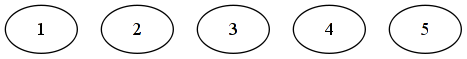
\includegraphics[width=0.6\textwidth]{images/randomgraph-01.png}
\caption{RandomGraph, stap 1}
\label{fig:randomgraph-01}
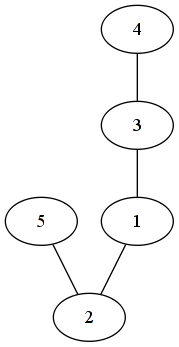
\includegraphics[width=0.3\textwidth]{images/randomgraph-02.png}
\caption{RandomGraph, stap 2}
\label{fig:randomgraph-02}
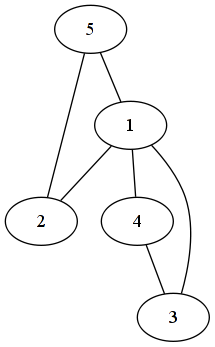
\includegraphics[width=0.3\textwidth]{images/randomgraph-03.png}
\caption{RandomGraph, stap 3}
\label{fig:randomgraph-03}
\end{center}
\end{figure}

\section{Het na\"ieve algoritme}

\subsection{Lazy genereren van embeddingen}
Ons na\"ieve algoritme overloopt alle embeddingen. Het is echter belangrijk dat
we de embeddingen op een \emph{lazy} manier genereren. Indien we de permutaties
\emph{strict} zouden genereren, zouden we een algoritme krijgen dat (weliswaar
met branching) het volgende idee implementeerd:

\lstset{language=Python}
\begin{lstlisting}
genus = +Infinity
for e in getEmbeddings(graph):
    eGenus = getGenus(e)
    if eGenus < genus:
        genus = eGenus
\end{lstlisting}

Hierbij is het probleem dat we pas informatie over het genus krijgen op het
moment dat e gegenereerd is. Als we hierop bounding criteria willen toepassen,
zouden we enkel de bladeren in onze zoekboom kunnen schrappen. Omdat we meer
willen schrappen, zoeken we dus naar een beter algoritme, waarin we vroeger
informatie over het genus verkrijgen.
\newline

\subsection{findGenus en findFaces}
Het genus van een graaf en een embedding $i$ wordt gegeven door
$v + f_i - e = 2 - 2g_i$. We weten $v$ en $e$ vast liggen, en enkel $f$ vari\"eert
als voor een graaf de embeddingen aflopen. Het zoeken van $min(g)$ komt dus
neer op het zoeken van $max(f)$, want
\begin{equation*}
min(g) = 1 - \frac{v + max(f) - e}{2}
\end{equation*}

\subsection{Algoritme: Het zoeken van het maximaal aantal vlakken}
Eerst zetten we de graaf die we krijgen als input om in een gerichte graaf. We
beginnen met een willekeurige (gerichte) boog $e_1$ die nog niet in een pad
ligt.  Stel dat op het einde van deze boog de top $v$ ligt. We nemen nu de
verzameling kandidaat bogen $E_v$ die op $e_i$ kunnen volgen. Deze stap is niet
triviaal en wordt verder beschreven in \ref{kandidaatbogen}. Nu moeten we branchen
voor elk element van $E_v$. We voegen de gekozen boog $e_{i+1}$ toe aan ons pad.
Indien deze boog dezelfde boog is als de eerste boog in ons pad, $e_1$, Hebben
we van ons pad een cykel gemaakt. Op dat moment kijken we of er nog bogen zijn
die niet in een pad liggen. Als dit het geval is, beginnen we een nieuw pad met
een willeukerige boog. Anders hebben we een volledige embedding gevonden, en
bevinden we ons in een blad van de zoekboom.
\newline

In pseudocode:
\lstset{language=Python}
\begin{lstlisting}
def findFaces(graph):
    return findFaces(graph, None, 0)

def findFaces(graph, currentPath, currentFaces):
    # No current path. Either we are done, or we have to start a new path.
    if currentPath is None:
        # Get a random vertex with some candidates.
        vertex = graph.getVertexWithCandidates()

        # No vertex found, this means we are done.
        if vertex is None:
            return currentFaces

        # Continue with a random edge.
        candidate = vertex.getRandomCandidate()
        edge = Edge(vertex, candidate)
        return findFaces(graph, [edge], currentFaces)

    # We need to branch for all candidates.
    else:
        # Retrieve the candidates.
        candidates = edge.getCandidates(currentPath.lastEdge())
        max = 0
        for candidate in candidates:
            if
            /* Connect the edge. */
            if(!currentVertex.connect(lastVertex, candidate)) {
                return currentFaces;
            }

            /* Check if we created a circle, which is the case if we are back in
             * our starting point and we can legally connect the cycle without
             * breaking any previous permutations. */
            if(candidate == cycleStart &&
                    cycleStart.connect(currentVertex, cycleSecond)) {
                /* Recurse with one more face found. */
                result = findFaces(graph, null, null, null, null,
                        currentFaces + 1, edgesLeft - 1, 0);

                /* Disconnect the cycle again. */
                cycleStart.split(currentVertex, cycleSecond);

            /* We did not create a cycle, so we just continue. */
            } else {
                result = findFaces(graph, cycleStart,
                        cycleSecond == null ? candidate : cycleSecond,
                        currentVertex, candidate, currentFaces,
                        edgesLeft - 1, edgesInCurrentCycle + 1);
            }

            /* We're only interested in the maximum number of faces we can find
             * in the graph. */
            if(result > max)
                max = result;

            /* Disconnect the cycle again. */
            currentVertex.split(lastVertex, candidate);
        }

        /* Return the solution with the most cycles. */
        return max;
    }
}
\end{lstlisting}

\subsection{Het nemen van kadidaatbogen volgend op een boog}
\label{kandidaatbogen}
Onze embedding defini\"eert voor elke top een bepaalde volgorde van de bogen in
deze top. We slaan deze volgordes op in de klasse \verb#CycleNode#. Initieel kan
elke boog volgen op elke andere boog. We stellen dit voor als $n$ deelvolgordes
\begin{equation*}
(e_1) (e_2) (e_3) \dots (e_n)
\end{equation*}
voor een top met $n$ bogen. Stel dat we op een bepaald moment in ons algoritme
in de top toekomen via $e_i$ en weggaan via $e_j$. Vanaf dit moment moeten we
hiermee rekening houden, mochten we nog eens in de top komen. We slaan dit op
als
\begin{equation*}
(e_1) (e_2) (e_3) \dots (e_i e_j) \dots (e_n)
\end{equation*}
Hoe vinden we nu de kandidaatbogen? Stel dat we uit $e_i$ komen. We hebben in
onze top de volgende volgordes opgeslaan:
\begin{equation*}
(e_{a1} e_{a2} \dots e_{ax}) (e_{b1} e_{b2} \dots e_{by}) \dots (e_{c1} e_{c2} \dots e_{cz})
\end{equation*}
We weten dat er nog geen boog volgt op $e_i$, dus zal $e_i$ het laatste element
zijn in een deelvolgorde.
\newline

We kunnen bijvoorbeeld niet $e_{a2}$ als volgende boog kiezen, omdat we al
gedefini\"eerd hebben dat deze op $e_{a1}$ volgt. Stel dat $e_i = e_{ax}$,
dan kunnen we niet als volgende boog $e_{a1}$ kiezen, want op dat moment zouden
we de deelvolgorde \emph{sluiten}. Dit mag niet, want, zoals in de opgave
beschreven wordt, moeten we uiteindelijk een volgorde als $(e_1 e_2 \dots e_n)$
uitkomen, zodat als we de volgorde doorlopen, elke $e$ tegenkomen.
\newline

Meer algemeen zijn de deelkandidaten die kunnen volgen op $e_i$ alle $e_j$ die
voldoen aan twee voorwaarden:
\begin{itemize}
\item $e_j$ is het eerste element van een deelvolgorde
$(e_j e_{j+1} ... e_{j+n})$.
\item $e_j$ zit niet in dezelfde deelvolgorde als $e_i$.
\end{itemize}

Een uitzondering bestaat wanneer we slechts \'e\'en deelvolgorde 
$(e_1 e_2 \dots e_i)$ ($e_i$ is dan het laatste element, aangezien het als
enige $e$ nog geen opvolger heeft) meer hebben. Dit geval is echter triviaal,
dan is de enige kandidaat $e_1$.

\end{document}
